\documentclass[12pt, a4paper, notitlepage]{report}
\usepackage{mathptmx}
\usepackage[T1]{fontenc}
\usepackage[utf8x]{inputenc}
\usepackage[english]{babel}
\usepackage{graphicx}
\usepackage{float}
\usepackage{amsmath}
\usepackage{mathtools}
\usepackage{amsfonts}
\usepackage{enumerate}
\usepackage{subfigure}
\usepackage[caption = false]{subfig}
\usepackage[top=2.5cm, bottom=2.5cm, left=2cm, right=2cm]{geometry}
\usepackage[font={small,it}]{caption}
\usepackage{fancyhdr}
\usepackage{listings}
\usepackage{color}
\usepackage{verbatim}

%\graphicspath{ {./Res\_L5\_k10/} {./Res\_L5\_k100/} {./Res\_L5\_k1000/} {./Res\_L10\_k10/} {./Res\_L10\_k100/} {./Res\_L10\_k1000/} {./Res\_L15\_k10/} {./Res\_L15\_k100/} {./Res\_L15\_k1000/} }

\definecolor{dkgreen}{rgb}{0,0.6,0}
\definecolor{gray}{rgb}{0.5,0.5,0.5}
\definecolor{mauve}{rgb}{0.58,0,0.82}
\definecolor{lyellow}{rgb}{1,1,0.9}

\lstset{backgroundcolor=\color{lyellow},
	frame=tb,
	language=Fortran,
	aboveskip=3mm,
	belowskip=3mm,
	showstringspaces=false,
	columns=flexible,
	basicstyle={\small\ttfamily},
	numbers=none,
	numberstyle=\tiny\color{gray},
	keywordstyle=\color{blue},
	commentstyle=\color{dkgreen},
	stringstyle=\color{mauve},
	breaklines=true,
	breakatwhitespace=true,
	tabsize=3
}

\pagestyle{fancy}
\lhead{Tommaso Tabarelli}
\chead{\thepage}
\rhead{\today}
\cfoot{Information theory and computation}
\rfoot{A.y. 2019/2020}
\lfoot{Exercise 9}

\begin{document}

\begin{center}
	\LARGE{Quantum information and computation: homework 9}\\
	\Large{of Tommaso Tabarelli}
\end{center}


\begin{abstract}
	In this homework we are asked to analyze a system of N spin-1/2 particles in a one-dimensional lattice. We should write the given Hamiltonian in a proper form and draw conclusions analyzing its spectrum.
\end{abstract}

\section*{Theory}

The N spin-1/2 particles system is described by the following hamiltonian:
\begin{equation}
\hat{H} = \lambda \sum_{i}^{N} \hat{\sigma}_z^i + \sum_{i}^{N-1} \hat{\sigma}_x^i \hat{\sigma}_x^{i+1}
\end{equation}
To be able to write down the hamiltonian in a matrix form, a basis shuold be chosen. For simplicity of representation, the z-component spin basis was chosen. Thus, it holds:
\begin{equation}
	\hat{\sigma}_z = \left(
	\begin{matrix}
		1 & 0 \\
		0 & -1
	\end{matrix} \right)
	\quad
	\hat{\sigma}_x = \left(
	\begin{matrix}
		0 & 1 \\
		1 & 0
	\end{matrix}
	\right)
\end{equation}
To go on, an important fact to notice is the implicit dimension of the $\sigma$s: every spin is implicitely immerged in the whole system space, thus it is represented by the tensor product between the identity matrices of other subsystems $\mathbb{I}_2^i$ and its own spin operator $\sigma_{x/z}$:
\begin{equation}
\sigma_z^i = \mathbb{I}^1 \otimes \mathbb{I}^2 \otimes ... \otimes \sigma_z^i \otimes ... \otimes \mathbb{I}^N
\end{equation}
and the interaction term results:
\begin{equation}
	\sigma_x^i \sigma_x^{i+1} = \mathbb{I}^1 \otimes \mathbb{I}^2 \otimes ... \otimes \sigma_x^i \otimes \sigma_x^{i+1} \otimes ... \otimes \mathbb{I}^N
\end{equation}

The system is not separable. Using a \textit{mean field} approximation we can estimate the energies. In this framework it holds:
\begin{equation}
	E[\psi_{MF}] = \langle \psi_{MF} \rvert H \lvert \psi_{MF} \rvert = \sum_{j=1}^{N-1} \langle \psi_{MF} \rvert \sigma_x^j \lvert \psi_{MF} \rangle^2 + \lambda \sum_{i=1}^{N} \langle \psi_{MF} \rvert \sigma_z^i \lvert \psi_{MF} \rangle
\end{equation}
and, in the termodynamic limit $N \to \infty$ it holds:
\begin{equation}
	e[\psi] = \frac{E[\psi]}{N} \underset{N \to \infty}{=} \langle \psi_{MF} \rvert \sigma_x \lvert \psi_{MF} \rangle^2 + \lambda \langle \psi_{MF} \rvert \sigma_z \lvert \psi_{MF} \rangle
\end{equation}
To find the ground state of the system the minimum of this quantity has to be find. It is found that:
\begin{equation}
	e = \begin{cases}
	-1 - \frac{\lambda^2}{4} & \quad \lambda \in [-2;2] \\
	-\lvert \lambda \rvert & \quad \lambda \notin [-2;2]
	\end{cases}
\end{equation}


\section*{Code development}
The Fortran program reads the number of particles and the dimension of them from two files and checks that they are reasonable (i.e. greater than 0).

To evaluate a general tensor product, a function has been defined in an external module called \textit{my\_math} in which there are also other functions from previous exercises.

In the program, the first part of the hamiltonian matrix is evaluated as a vector. It is then stored in an auxiliary variable called \textit{hamilt\_magn}.

\begin{lstlisting}
! Building diagonal
DO ii=1,num_par
	step = dim_**(num_par+1-ii)
	DO jj=0,dim_**num_par-1,step
		h_diag((jj+1):(jj+step/2)) = h_diag((jj+1):(jj+step/2))+1
		h_diag((jj+step/2+1):(jj+step)) = h_diag((jj+step/2+1):(jj+step))-1
	END DO
END DO

! Initializing hamiltonian of sigma_z contribute using the diagonal
!	representing the interaction
DO ii=1,dim_**num_par
	hamilt_magn(ii,ii) = h_diag(ii)
END DO
\end{lstlisting}

Next step was to evaluate the interaction part; following method was used:
\begin{itemize}
	\item an auxiliary matrix (called \textit{app}) having the same dimension of the hamiltonian was allocated;
	
	\item going on with evaluation, its first square section properly chosen was used (this section can never be greater than the whole hamiltonian);
	
	\item when the evaluation is finished, the auxiliary matrix is added to the another auxiliary matrix called \textit{hamilt\_int} and resetted to 0 to be ready for another iteration.
\end{itemize}

\begin{lstlisting}
! Looping over the interaction couples (which are N-1)
DO ii=1,num_par-1
	! Restoring the app variable
	app = 0
	! We have to evaluate only (N-1) tensor products (in case of dim^2, we have only 1 tensor product for example)
	!	The trick is to evaluate N tensor products, having the first one trivially evaluated
	DO jj=1,num_par
		! If first step, then do "trivial evaluation"
		IF (jj.EQ.1) THEN
			! The interactions are between particle ii and ii+1
			IF (((num_par+1-jj).EQ.ii).OR.((num_par+1-jj).EQ.(ii+1))) THEN
				app(1:dim_**(jj),1:dim_**(jj)) = sigma_x(:,:)
				! Debugging
				WRITE(*,*) "sigma_x"
			ELSE
				app(1:dim_**(jj),1:dim_**(jj)) = ident_2(:,:)
				! Debugging
				WRITE(*,*) "ident_2"
			END IF
		ELSE
			! The interactions are between particle ii and ii+1
				IF (((num_par+1-jj).EQ.ii).OR.((num_par+1-jj).EQ.(ii+1))) THEN
				! Storing increasing matrices to evaluate the temporary results
				app(1:dim_**(jj),1:dim_**(jj)) = Tensor_product(sigma_x, app( 1:dim_**(jj-1),1:dim_**(jj-1) ))
				! Debugging
				WRITE(*,*) "sigma_x"
			ELSE
				app(1:dim_**(jj),1:dim_**(jj)) = Tensor_product(ident_2, app( 1:dim_**(jj-1),1:dim_**(jj-1) ))
				! Debugging
				WRITE(*,*) "ident_2"
			END IF
		END IF
	END DO
	
	WRITE(*,*) "--------------------------"
	
	! After having evaluated the temporary result, add it to the hamiltonian
	hamilt_int(:,:) = hamilt_int(:,:) + app(:,:)

END DO
\end{lstlisting}

After this, a loop over $\lambda$ parameter is done, using values $\in [0,3]$ updating $\lambda$ using steps of 0.15. In this loop the two auxiliary hamiltonians are added, the first multiplied by $\lambda$. The resulting hamiltonian is then diagonalized and the first four eigenvalues for each iteration are stored in a matrix.
At the end, the matrix is printed to a file with the respective $\lambda$ values at the beginning of each line.

\begin{lstlisting}
dimen = dim_**num_par

DO ii=0,20
	
	lambda = 3.0/(20.)*ii
	
	WRITE(*,*) "Evaluating lambda = ", lambda
	
	! Building proper hamiltonian
	hamilt = 0
	hamilt(:,:) =  hamilt_int(:,:) + lambda*hamilt_magn(:,:)
	
	! DIAGONALIZING
	! Allocating 1 value for wk_opt
	ALLOCATE(wk_opt(1))
	
	! Giving LWORK=-1 the subroutine only evaluates the optimal dimension for WORK_
	LWORK_=-1
	
	! See documentation online
	!  (http://www.netlib.org/lapack/explore-html/d2/d8a/group__double_s_yeigen_ga442c43fca5493590f8f26cf42fed4044.html) 
	CALL ZHEEV('N', 'U', dimen, hamilt, dimen, eig_val, wk_opt, LWORK_, RWORK_, info_eig)
	
	LWORK_ = INT(wk_opt(1))
	
	! Allocating the optimal dimension for WORK
	ALLOCATE(WORK_(LWORK_))
	
	! Recalling the subroutine to do the diagonalization	
	CALL ZHEEV('N', 'U', dimen, hamilt, dimen, eig_val, WORK_, LWORK_, RWORK_, info_eig)
	
	DEALLOCATE(wk_opt)
	DEALLOCATE(WORK_)
	
	! Storing the first four eigenvalues for every lambda
	eig_val_results(ii+1,1) = lambda
	eig_val_results(ii+1,2:5) = eig_val(1:4)

END DO

! ---------- STORING RESULTS ----------

! Saving eigenvalues to file
OPEN(12, file="eig_val_results.txt", status='REPLACE', action='WRITE')

DO ii=1,21
	WRITE(12,"(F12.8)",advance="No") eig_val_results(ii,1)
	
	DO jj=2,5-1
		WRITE(12,"(F15.8)",advance="No") eig_val_results(ii,jj)
	END DO
	
	WRITE(12,"(F15.8)",advance="Yes") eig_val_results(ii,5)
END DO

CLOSE(12)
\end{lstlisting}

The results are then plotted using gnuplot scripts.

\section*{Results}

The maximum nuber of particles was tested and it turned out to be $N=13$ ($N=14$ simply makes the command line says "\textit{killed}"). The program was run using increasing number of particles $N$.

The results are shown in the following images.

\begin{figure}
	\centering
	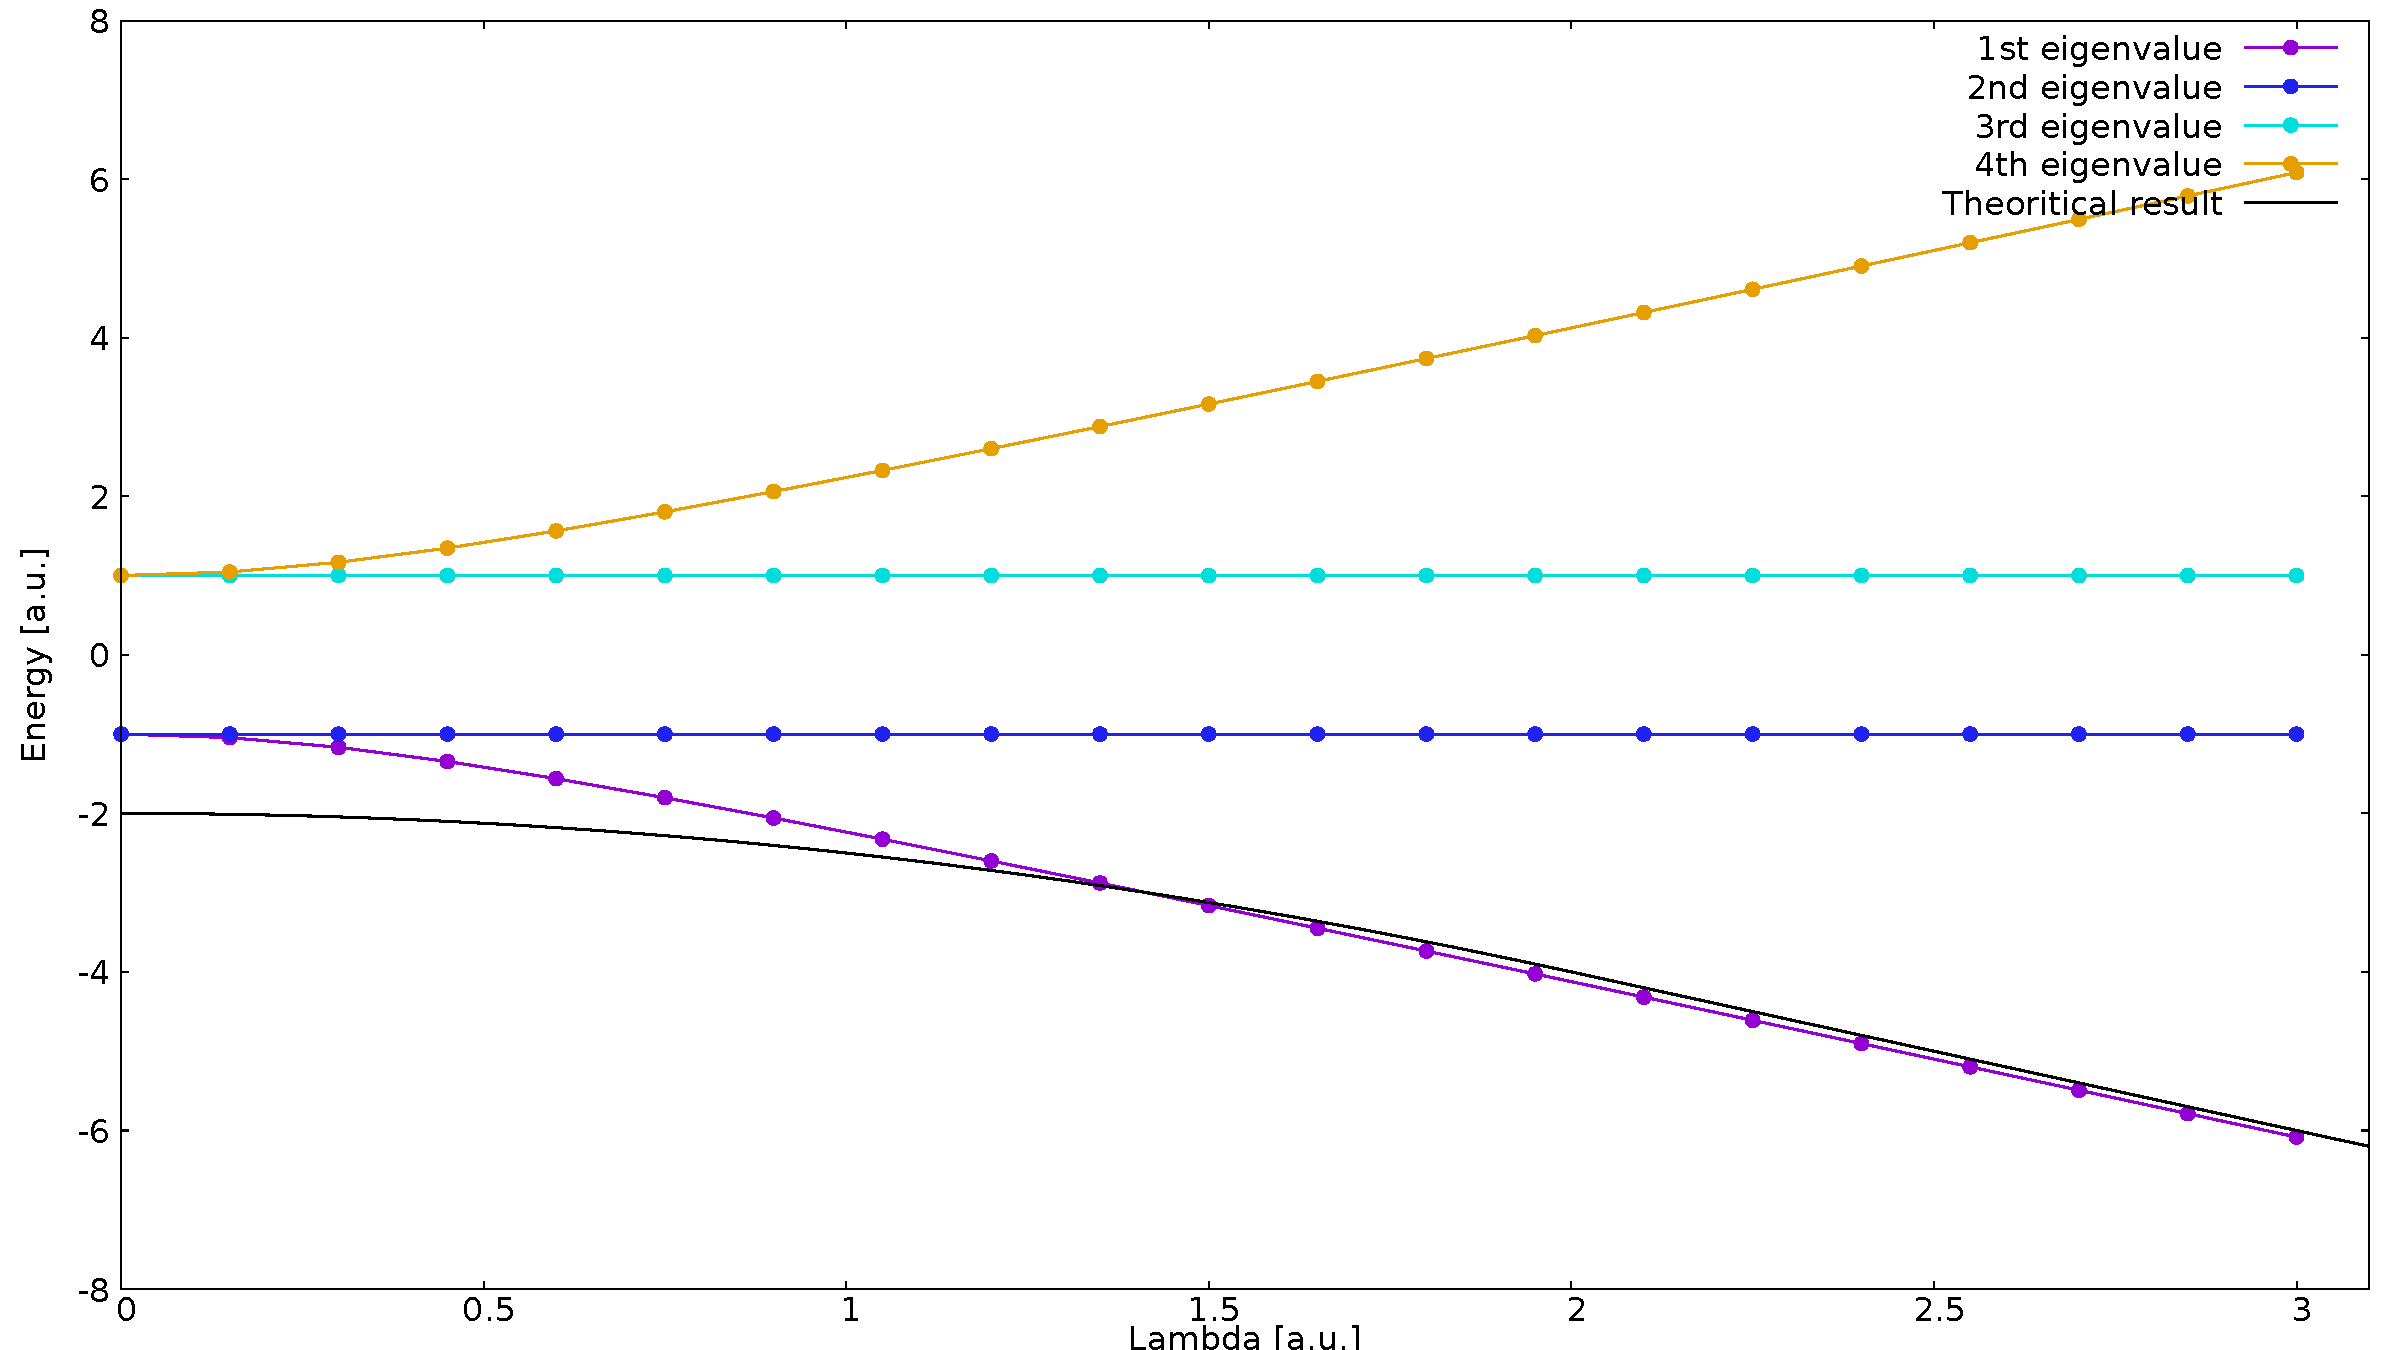
\includegraphics[scale=0.3]{4_eigval_vs_lambda_N2} 
	\caption{Hamiltonian eigenvalues vs $\lambda$ for N=2.}
	\label{figure_lambdas}
\end{figure}

\begin{figure}
	\centering
	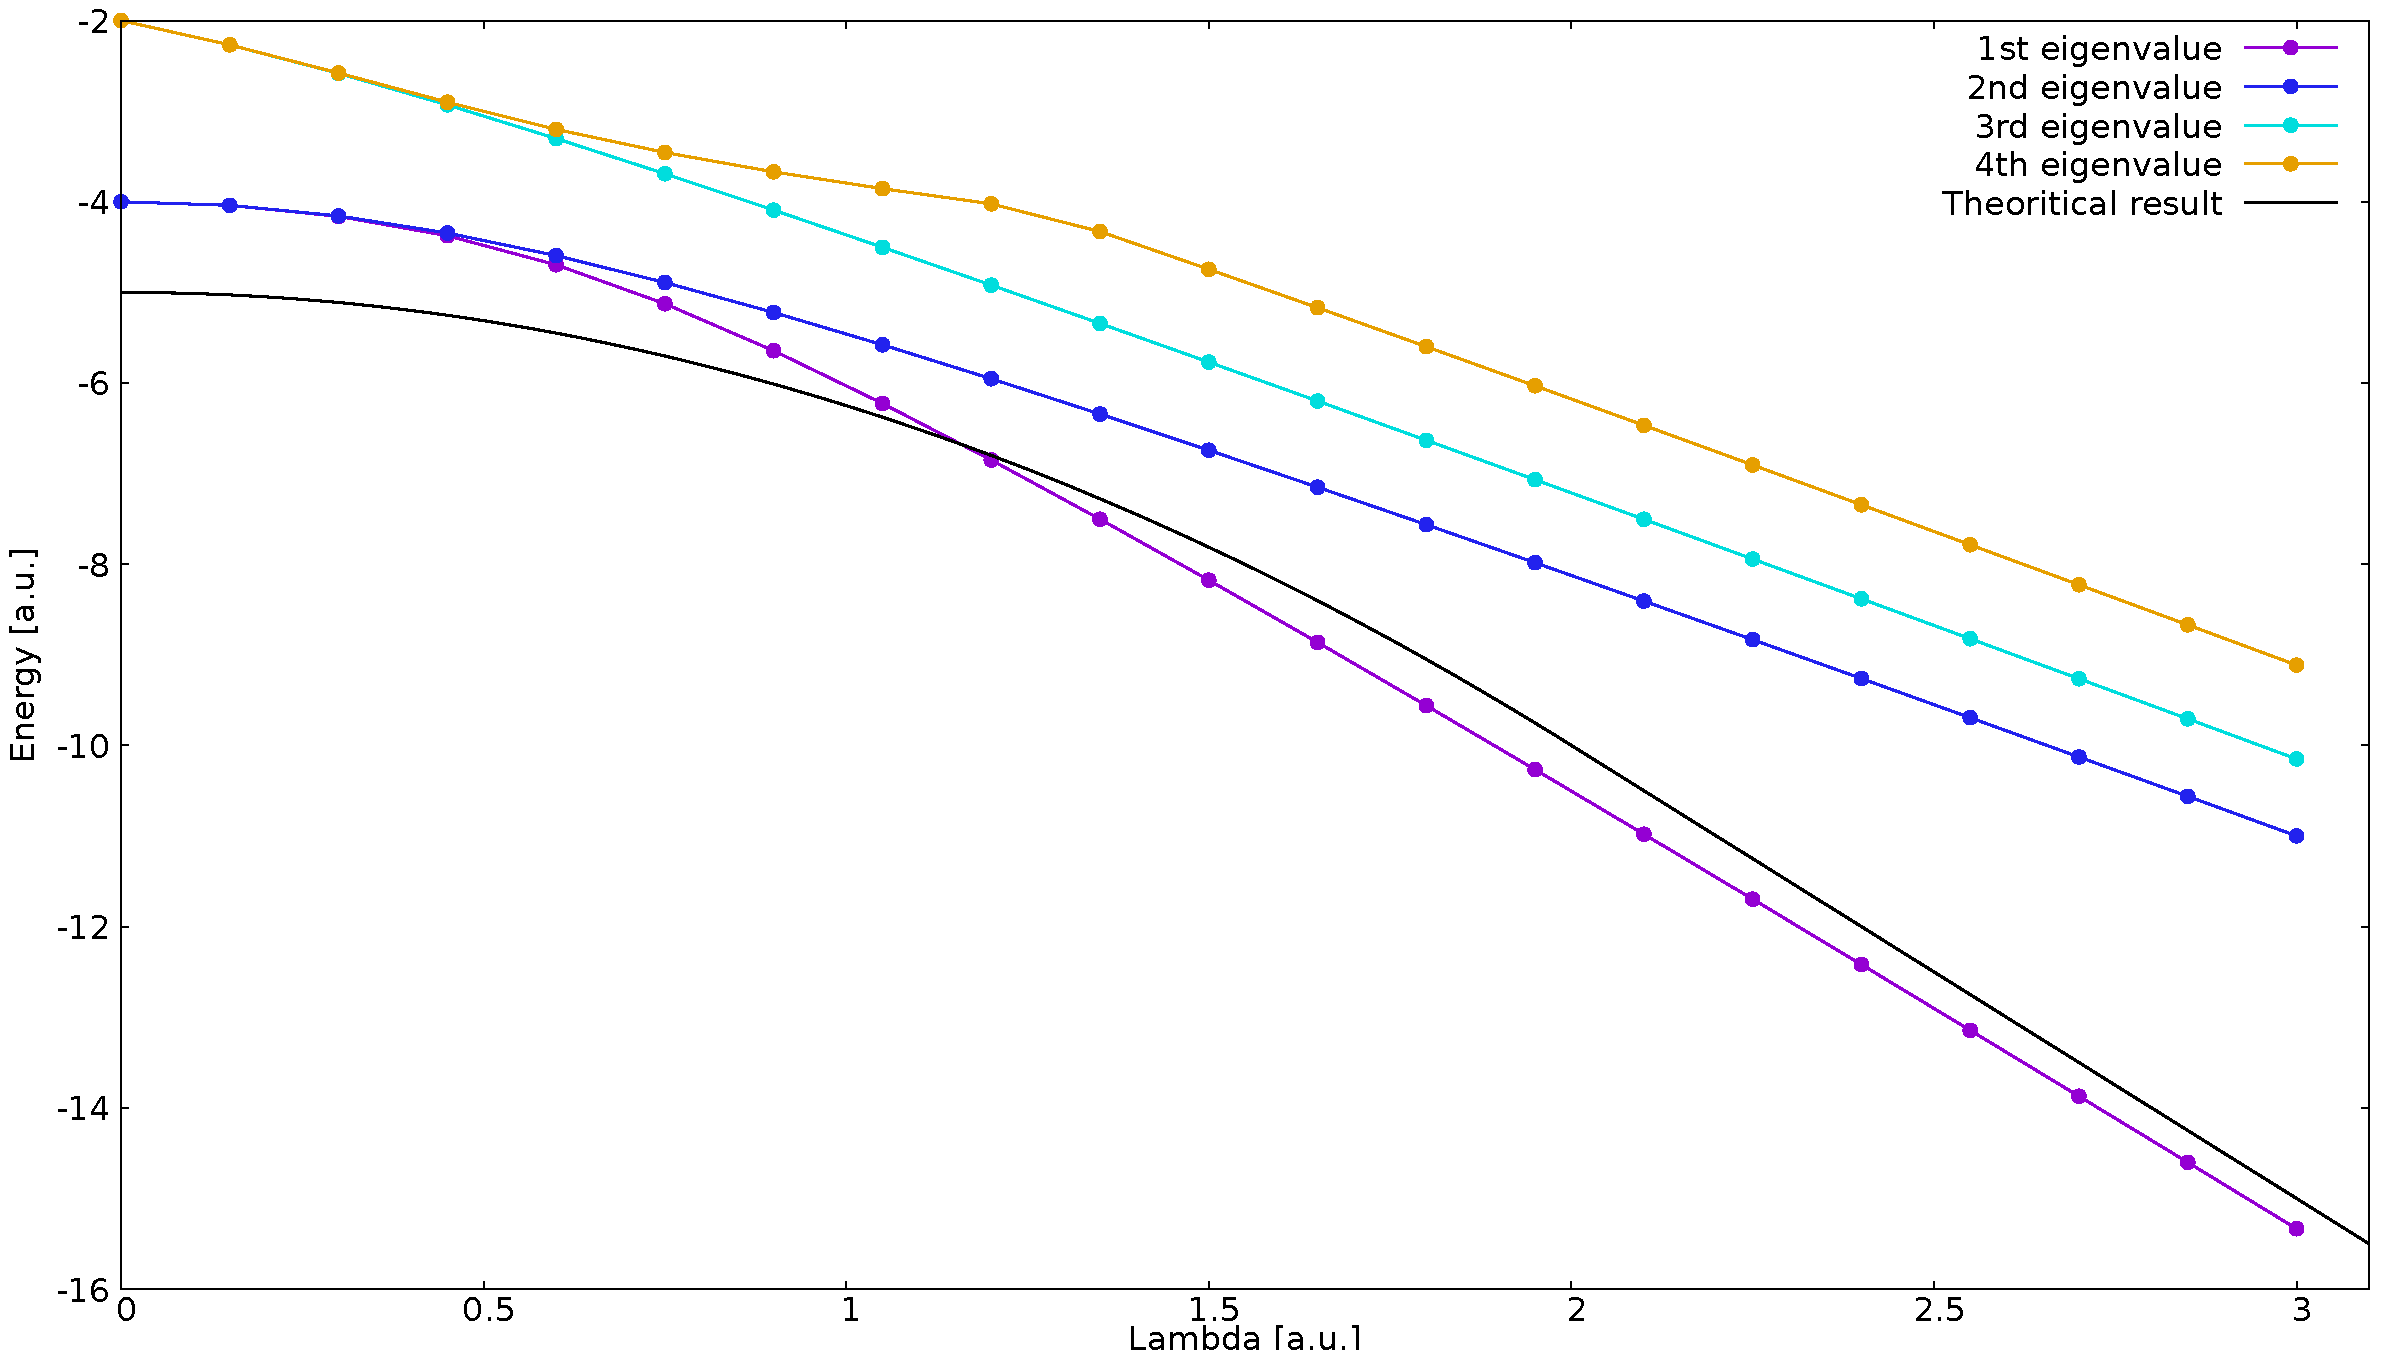
\includegraphics[scale=0.3]{4_eigval_vs_lambda_N5} 
	\caption{Hamiltonian eigenvalues vs $\lambda$ for N=5.}
	\label{figure_lambdas}
\end{figure}

\begin{figure}
	\centering
	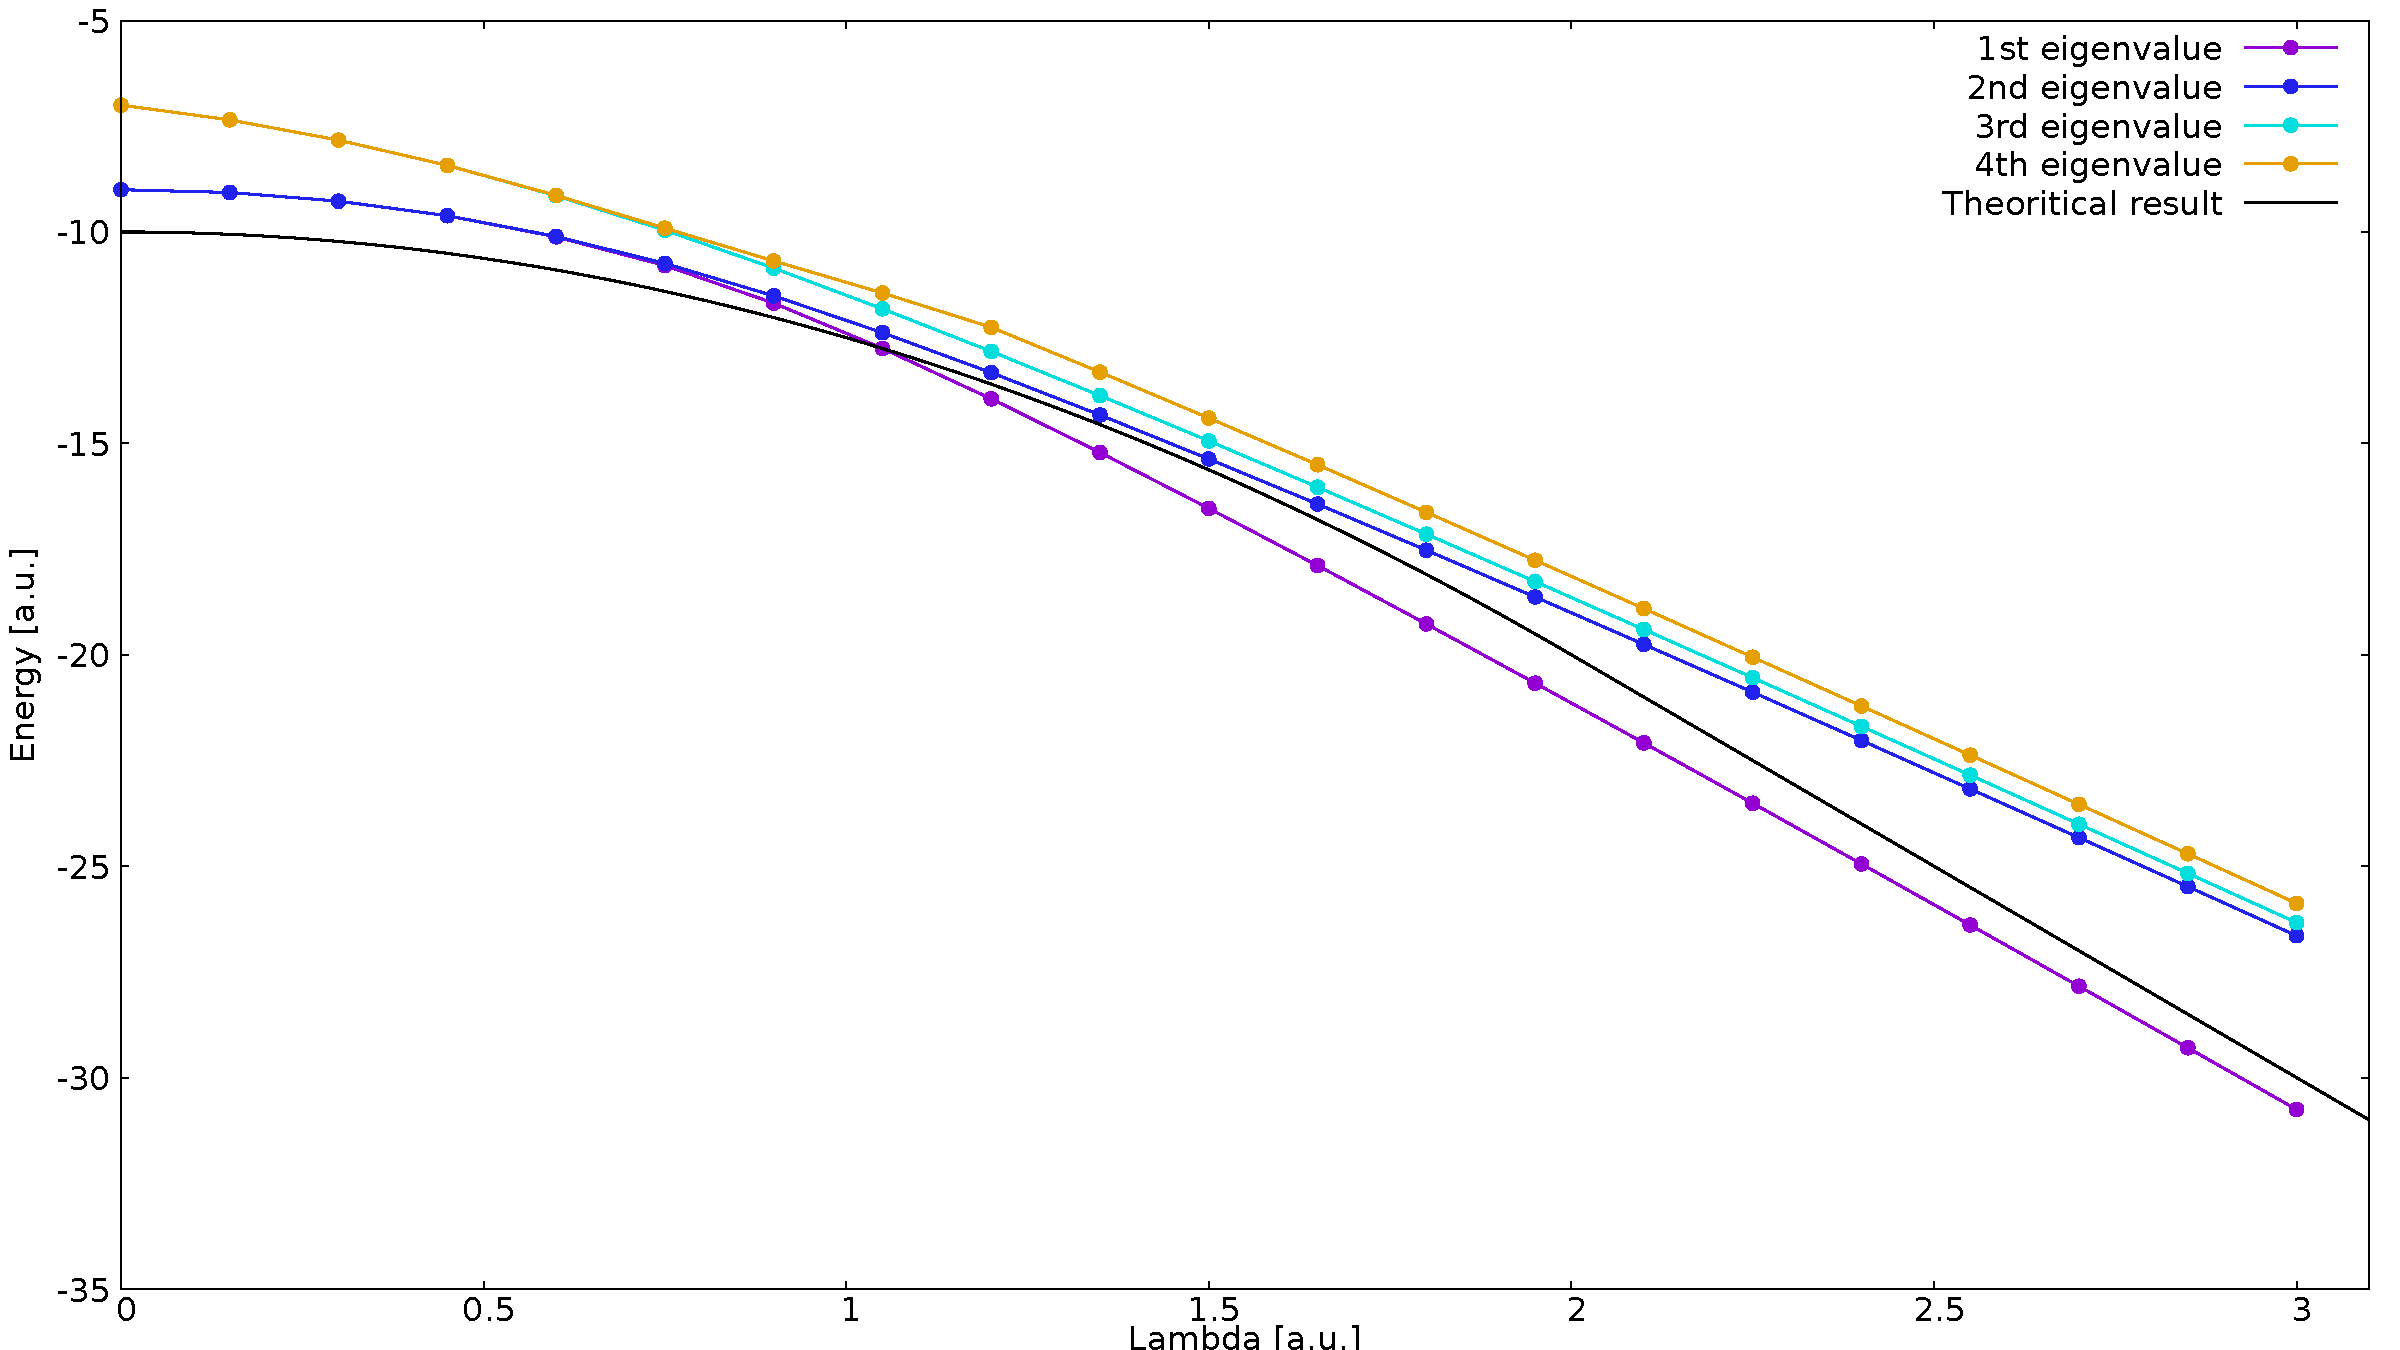
\includegraphics[scale=0.3]{4_eigval_vs_lambda_N10}
	\caption{Hamiltonian eigenvalues vs $\lambda$ for N=10.}
	\label{figure_lambdas}
\end{figure}

\begin{figure}
	\centering
	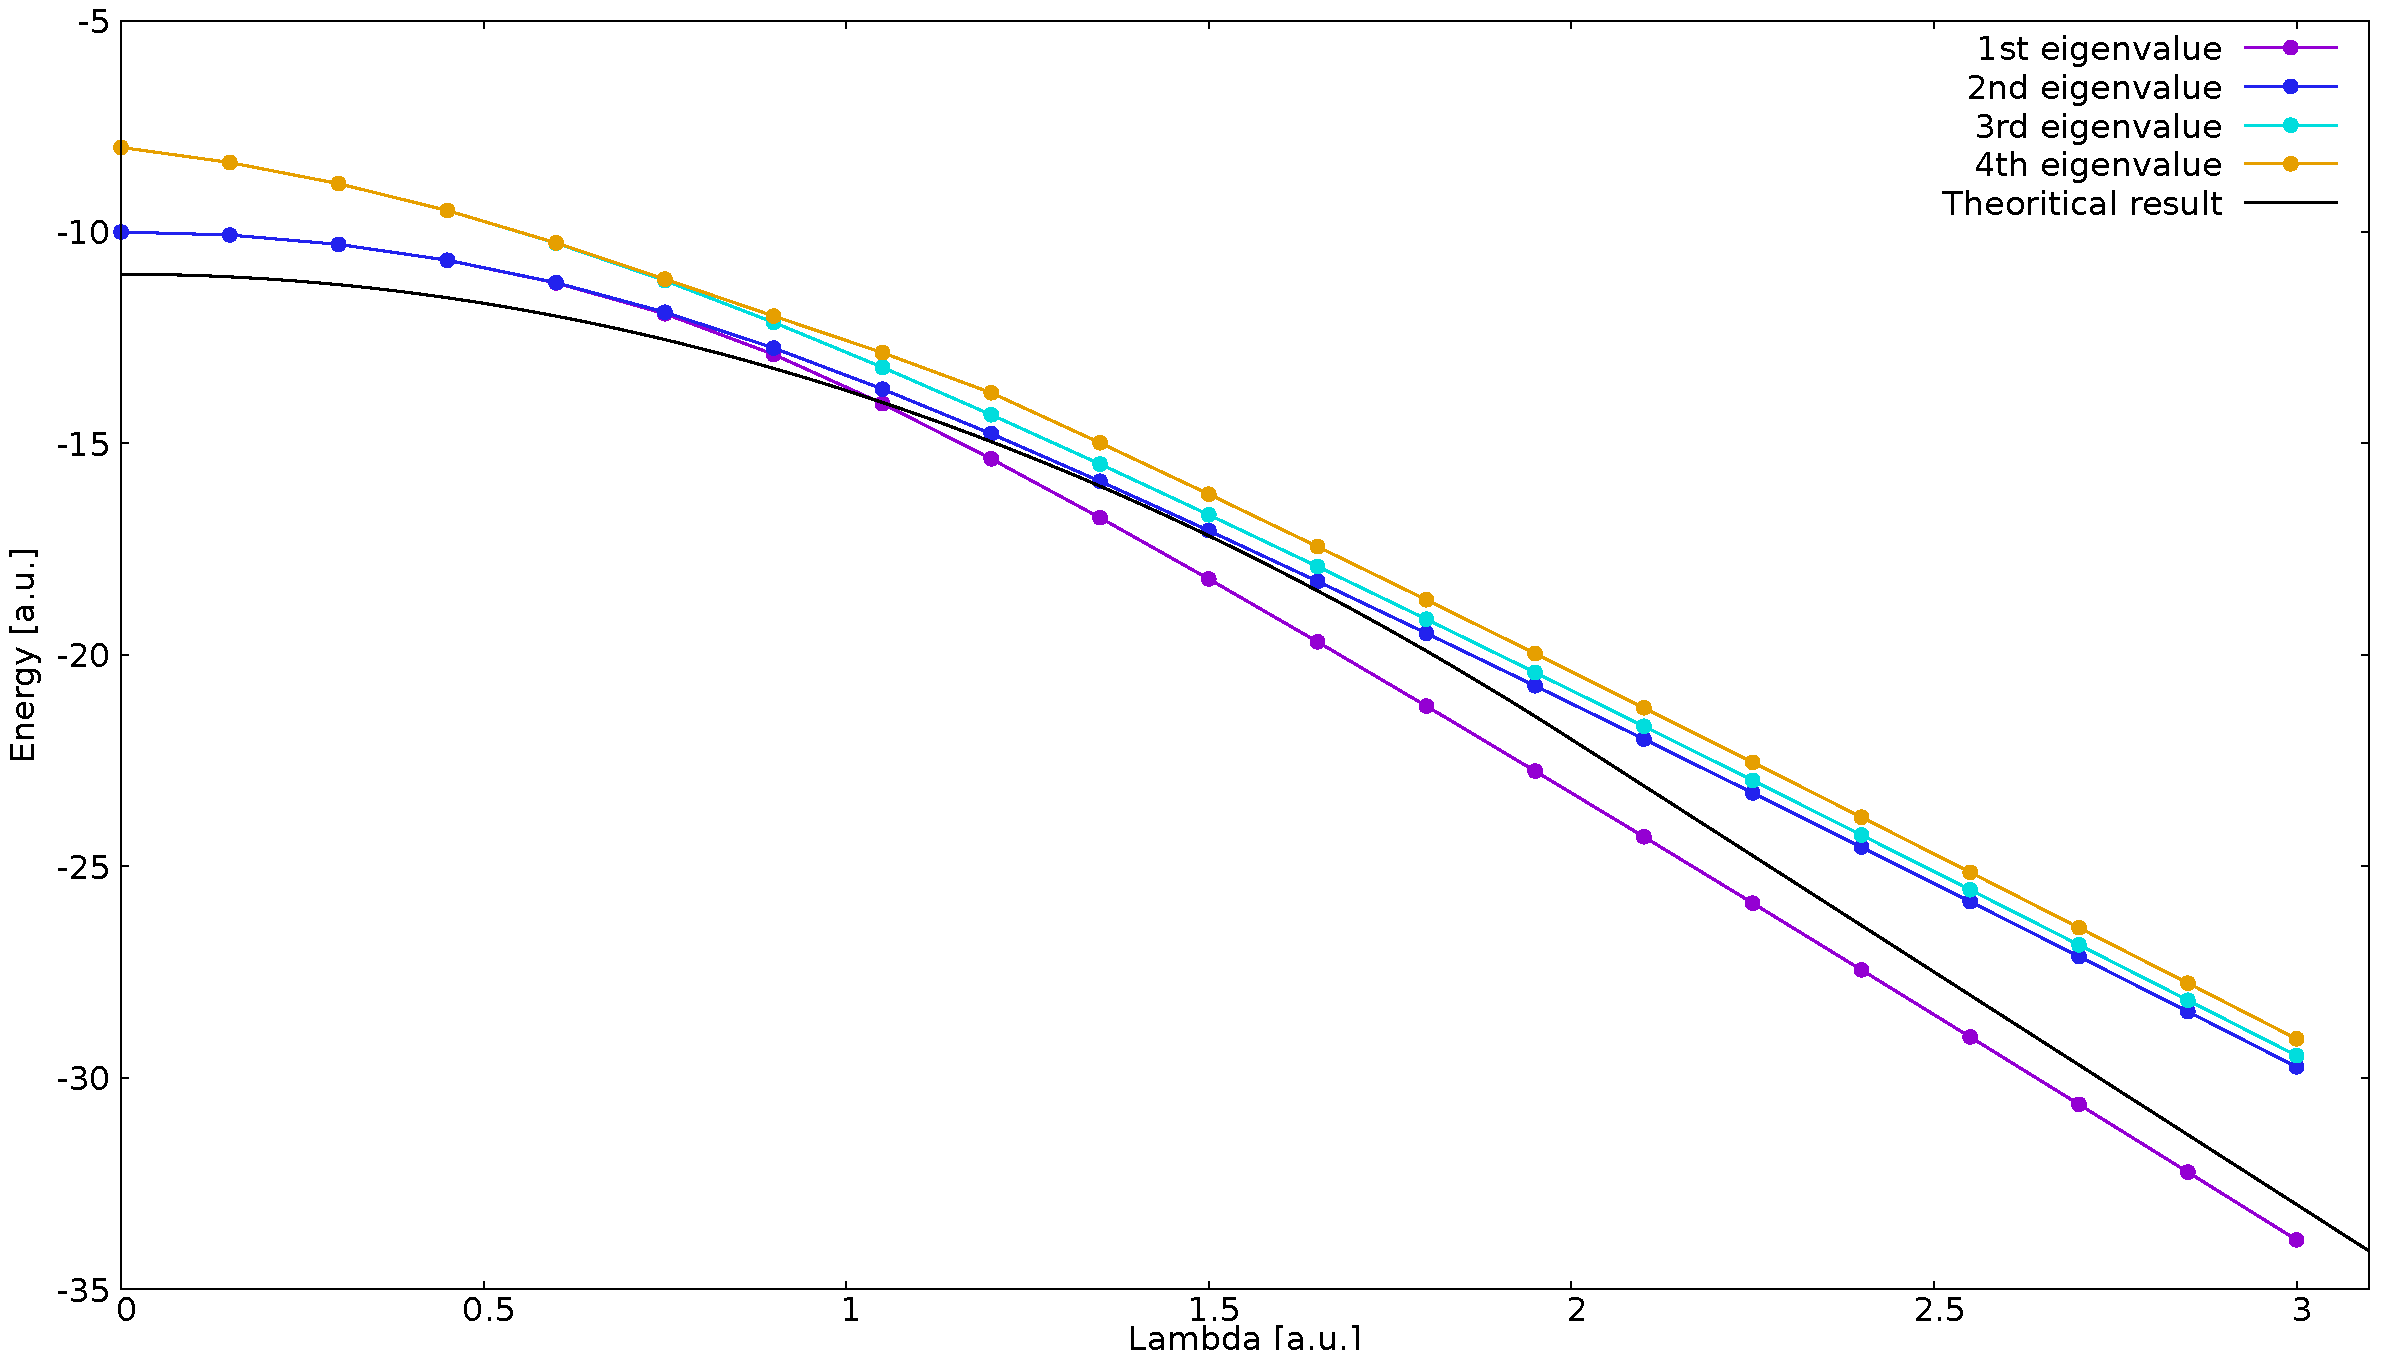
\includegraphics[scale=0.3]{4_eigval_vs_lambda_N11}
	\caption{Hamiltonian eigenvalues vs $\lambda$ for N=11.}
	\label{figure_lambdas}
\end{figure}

\begin{figure}
	\centering
	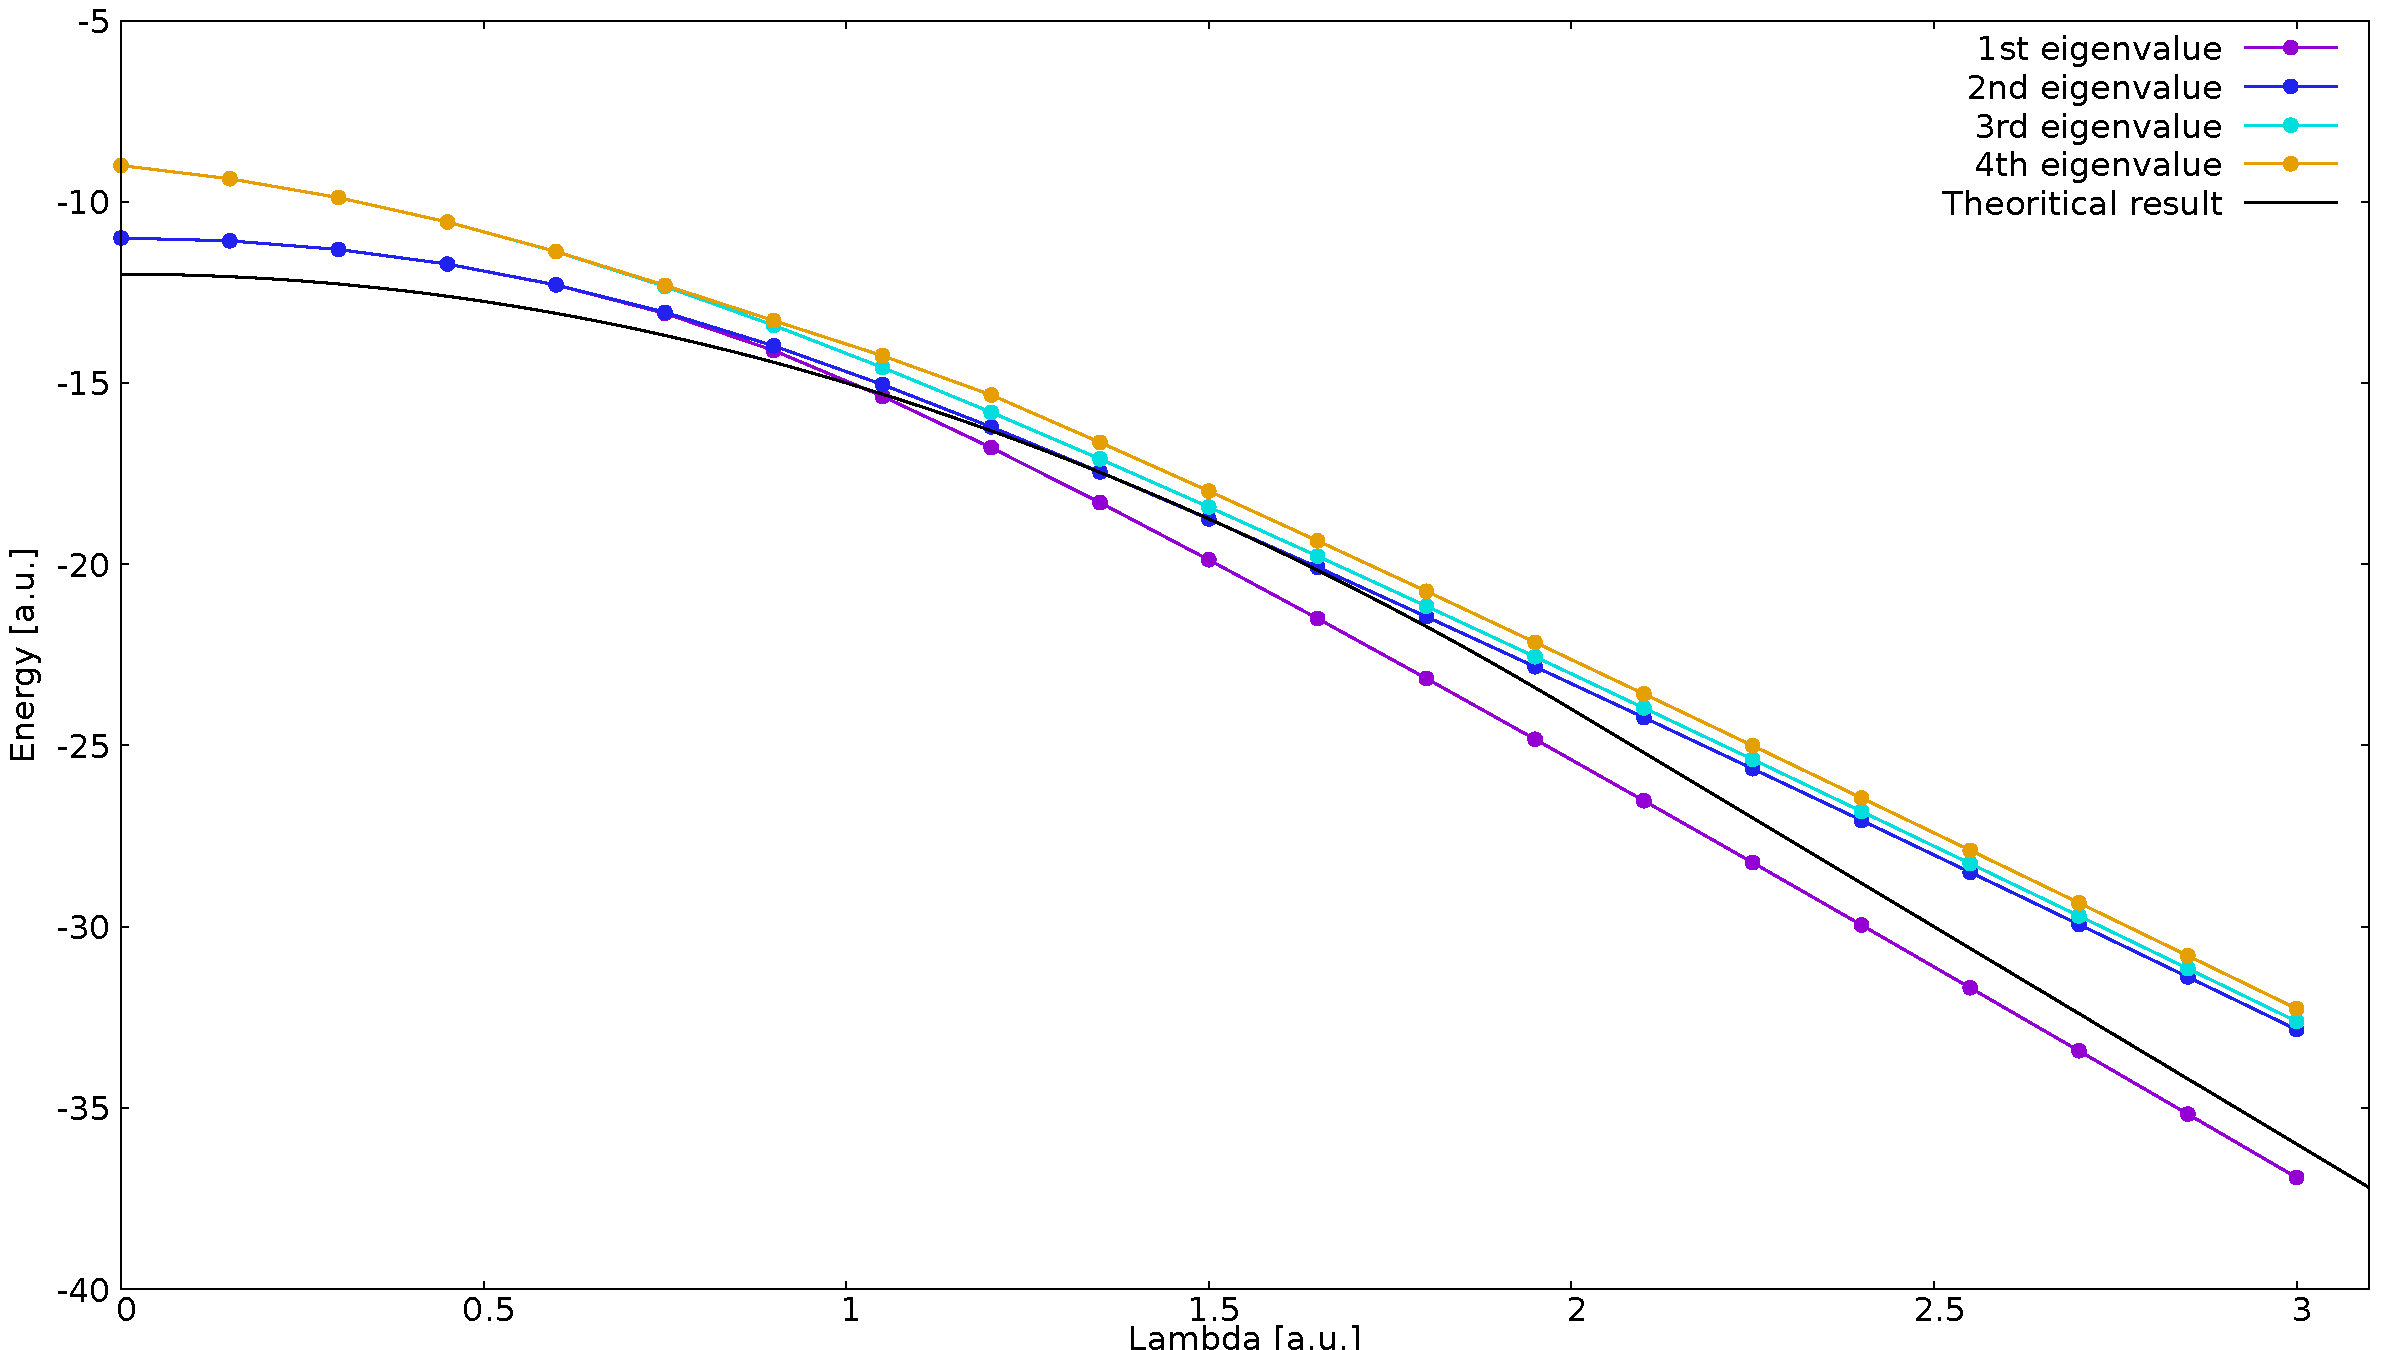
\includegraphics[scale=0.3]{4_eigval_vs_lambda_N12}
	\caption{Hamiltonian eigenvalues vs $\lambda$ for N=12.}
	\label{figure_lambdas}
\end{figure}

\begin{figure}
	\centering
	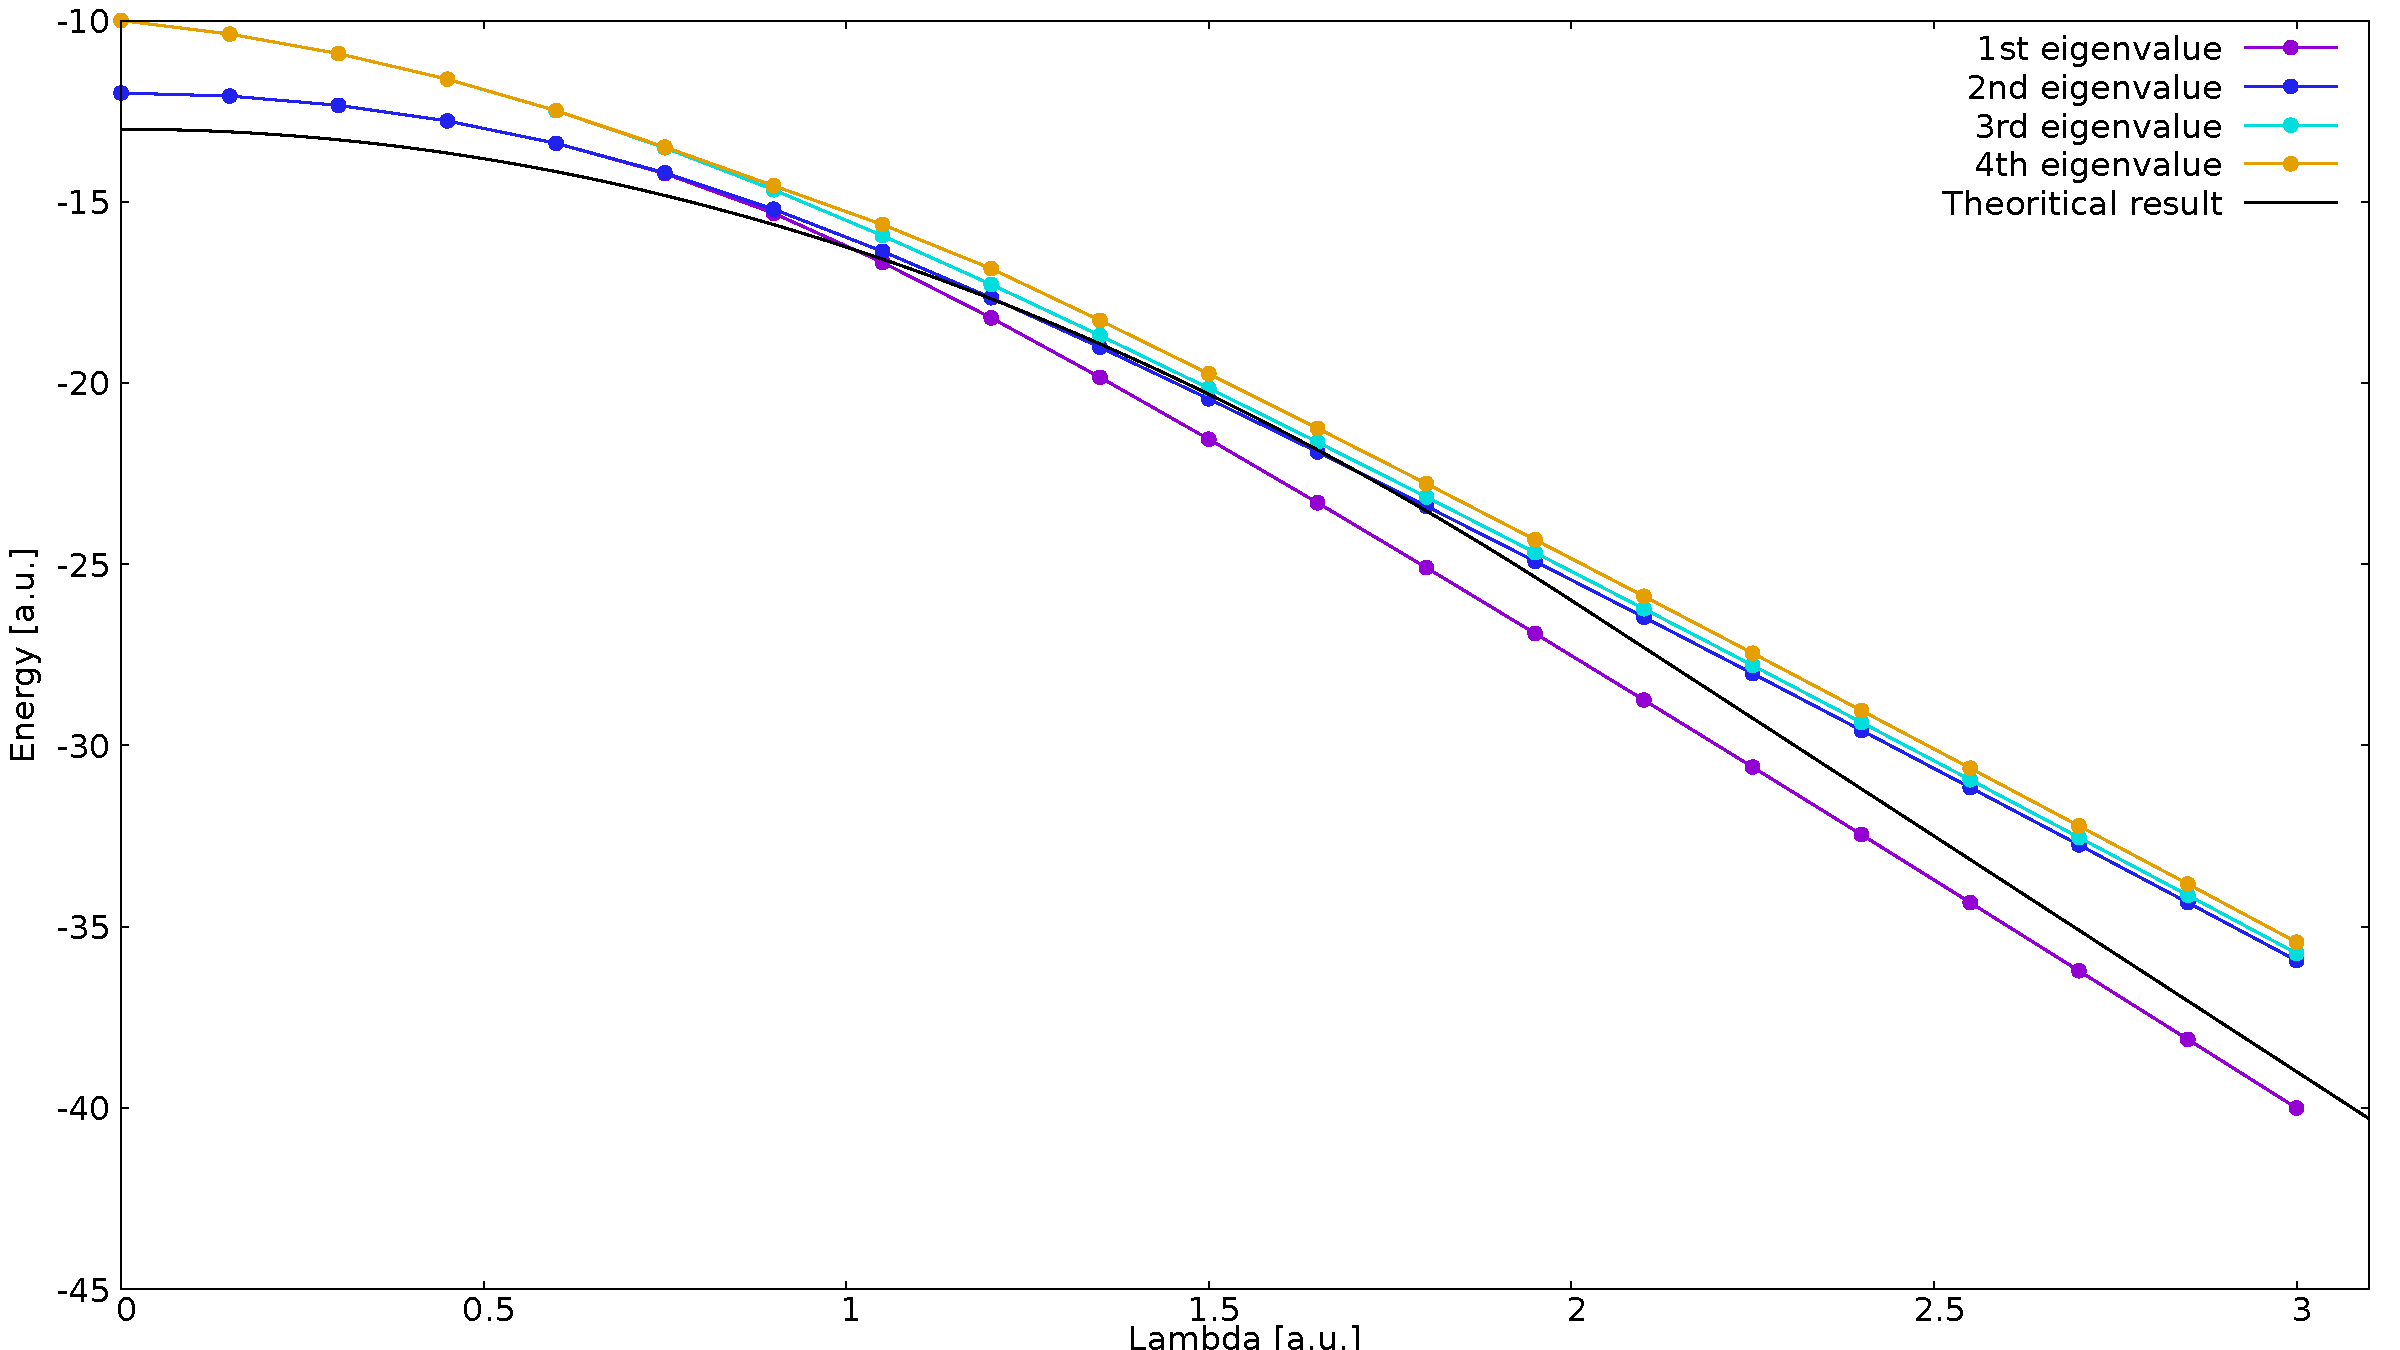
\includegraphics[scale=0.3]{4_eigval_vs_lambda_N13}
	\caption{Hamiltonian eigenvalues vs $\lambda$ for N=13.}
	\label{figure_lambdas}
\end{figure}

The considered hamiltonian is composed by two parts: the first one represents the z-component spin interactions with an external magnetic field $\lambda$ (more precisely, the interaction with the z-component of such a field) while the second part is that of an antiferromagnetic system.

Before going further, let us adopt a change of notation: "$\pm$1/2" spins will be denoted using "$\pm$1".

The ground state of the first part alone is a state in which all the z-components of the spins are directed as the external field but have opposite orientation. The ground state of the second system (in absence of an external field) is that where all the spins alternate their x-components, thus reaching a minimum of the energy. This state is degenerated since there are two configurations that make it possible: one where the "first" spin has x-component equal to +1 (and all the others have their x-components alternated: so $\sigma_x^{i=2} = -1, \sigma_x^{i=3} = +1$ and so on), the other having the first x spin component set to +1.

The second energy state for the first system is that when one single spin is oriented in the same way as the external field: this state has degeneration equal to the number of particles $N$ since it can be achieved in turning one single spin in N different ways. The second energy state of the second subsystem is reached when one single interaction "breaks the alternance chain", for example in the chain $\sigma_x^{i=1} = -1, \sigma_x^{i=2} = +1, \sigma_x^{i=3} = -1, ... , \sigma_x^{i=2k-1} = -1, \sigma_x^{i=2k} = -1, \sigma_x^{i=2k+1} = +1, ...$ the $\sigma_x^{i=2k} = -1$ is the opposite of that expected, and after it all the others are reversed (so that one single interaction term is reversed). Straightforward, the degeneration of this state is $N-1$ since there can be $N-1$ different interactions that can be changed to pass from the ground state to the second one.

The spectrum of the system represent the energy levels accessible by the system itself. When the $\lambda$ parameter is equal to 0 the system is described only by the second part of the hamiltonian thus showing the behaviour aforementioned with the first two eigenvalues being degenerated. With increasing $\lambda$ the system is described more likely by the first part of the hamiltonian, thus the first eigenvalue tends not to be degenerated. While passing from one to another a phase trainsition occurs. Specifically, it is a quantum phase trainsition because the system has a quantum nature.

This kind of behaviour is enlightened by the figures, where the passage of the second eigenvalue from the first "group" of (degenerated) eigenvalues to the second one with increasing $\lambda$ states the changing in the nature of the system.

\section*{Self-evaluation}
In this task I learned how to model a $N$ 1/2-spin particles system. I also learned hamiltonian main features and reflected on hamiltonian spectrum, understanding that a quantum phase transition is being observed when $\lambda$ is changing.

\subsection*{Correctness}

My program does what is expected to do, but as aforementioned, it works only untill $N=13$.

There are no compilation problems.

Pre- and post-conditions and checkpoints are not used so much due to the large amount of time they require to be implemented (compared to the time we have to do the task).

\subsection*{Stability}

There are loops made on non integers variables, but there is no specific check that can lead to "weird errors".

Maybe some memory error can arise if the space dimension $d$ or the number of particles $N$ (or even both parameters) become too large due to the fact that the matrix dimension goes as $d^{2N}$.

\subsection*{Accurate discretization}

There is no particular discretization issues.

\subsection*{Flexibility}

I tried to comment as much as possible the code so to have a clear and understandable code.

\subsection*{Efficiency}

Diagonalization routine is not implemented by hand. For what concerns memory and time usage, they depend on the parameters passed.\\ \\

My work can be improved: for example, $\lambda$ range can be passed as input. Moreover, the routine used to evaluate the matrix tensor product can be substituted by a \textit{ad hoc} algorithm for this specific case.

\end{document}